\chapter{Chow-Liu Trees
and Tree Augmented Naive Bayes (TAN)}
\label{ch-chow}

This chapter is mostly based
on chapter 8 of Pearl's 1988 book
Ref.\cite{pearl-1988book}. See also 
Ref.\cite{wiki-chow} and references
therein.

This chapter uses various Shannon Information Theory
entropies. Our 
notation for these
entropies
is described in Chapter \nameref{ch-not-cons}
on Notational Conventions.

\section{Chow-Liu Trees}
Chow-Liu trees refers 
to an 
algorithm for finding
a bnet tree
that fits an a priori
given probability distribution
as closely as possible.


Consider a bnet with $n$ nodes
$\rvx^n=(\rvx_0, \rvx_1, \ldots, \rvx_{n-1})$
such that 
$\rvx_i\in S_{\rvx_i}$
for all $i$. Let its  
 total probability distribution be
$P_{\rvx^n}$. For
simplicity, we will abbreviate $P_{\rvx^n}$ by $P$.
Hence


\beq
P(x^n)=P_{\rvx^n}(x^n)
\;.
\eeq

Suppose we want to fit $P_{\rvx^n}$
by a tree bnet with nodes
$\rvt^n=(\rvt_0, \rvt_1, \ldots, \rvt_{n-1})$
such that
$\rvt_i\in S_{\rvt_i}=S_{\rvx_i}$
for all $i$.
 For
simplicity, we will abbreviate $P_{\rvt^n}$ by $P_T$.
Hence

\beq
P_T(x^n)=P_{\rvt^n}(x^n)
\;.
\eeq

Throughout this chapter, let
$V=\{0, 1, \ldots, n-1\}$, the set of vertices.
Suppose $\mu$ is a function
$\mu:V\rarrow V$
such that $\mu(i)< i$.
Let
$T_\mu=\{\rvt_{\mu(i)}\rarrow \rvt_i:
 i\in V-\{0\}\}$.
Then $T_\mu$
is a tree that spans (
i.e., it includes all nodes)
 $\rvt^n$.
Its root node 
is
$\rvt_0$, because $\rvt_0$ has no parents.
All other nodes $\rvt_i$ have exactly
one parent,
namely $ \rvt_{\mu(i)}$.
Let $P_T$,
the total probability 
distribution for 
the tree, be parameterized
by the function $\mu$
as follows:



\beq
P_T(x^n)=\prod_{i=0}^{n-1}
P_T(x_i|x_{\mu(i)})
\label{eq-pt-prod}
\;,
\eeq
where, for the root node 0, 
$P_T(x_0|x_{\mu(0)})=P_T(x_0)$.

\begin{claim}\label{claim-chow1}
$D_{KL}(P\parallel P_T)$
is minimized 
over all
probability
distributions
$P_T$ that are
expressible as 
Eq.(\ref{eq-pt-prod})
iff

\beq
P_T(x_i|x_{\mu(i)})
=
P(x_i|x_{\mu(i)})
\eeq
for all $i$, and

\beq
\sum_i H(\rvx_i:\rvx_{\mu(i)})
\eeq
is maximized over all $\mu$.
\end{claim}
\proof

\begin{align}
D_{KL}(P\parallel P_T)
&=
\sum_{x^n} P(x^n)\ln 
\frac{P(x^n)}{P_T(x^n)}
\\
&=
-\sum_{x^n}
\sum_i P(x^n)\ln 
P_T(x_i| x_{\mu(i)})
+
\sum_i P(x^n)\ln 
P(x^n)
\\
&=
-
\sum_i
\sum_{x_i, x_{\mu(i)}} P(x_i, x_{\mu(i)})\ln 
P_T(x_i| x_{\mu(i)})
-
H(\rvx^n)
\\
&=
-
\sum_i
\sum_{x_{\mu(i)}} 
P(x_{\mu(i)})
\left[
\sum_{x_i}
P(x_i| x_{\mu(i)})\ln 
P_T(x_i| x_{\mu(i)})
\right]
-
H(\rvx^n)
\;.
\end{align}
Now note that

\beq
\sum_{x_i}
P(x_i| x_{\mu(i)})\ln 
\frac
{P(x_i| x_{\mu(i)})}
{P_T(x_i| x_{\mu(i)})}
\geq 0
\eeq
and
this inequality
becomes an equality iff

\beq
P(x_i| x_{\mu(i)})=
P_T(x_i| x_{\mu(i)})
\;.
\label{eq-inherits-tpm}
\eeq
Therefore

\beq
D_{KL}(P\parallel P_T)
\geq
-
\sum_i
\underbrace{
\sum_{x_{\mu(i)}} 
P(x_{\mu(i)})
\left[
\sum_{x_i}
P(x_i| x_{\mu(i)})\ln 
P(x_i| x_{\mu(i)})
\right]
}_{=H(\rvx_i|\rvx_{\mu(i)})=
H(\rvx_i:\rvx_{\mu(i)})-H(\rvx_i)}
-
H(\rvx^n)
\;,
\eeq
and this inequality
becomes an equality iff
Eq.(\ref{eq-inherits-tpm})
is satisfied.

Note from the last
equation that

\beq
\argmin_\mu D_{KL}(P\parallel P_T)=
\argmax_\mu
\sum_i H(\rvx_i:\rvx_{\mu(i)})
\;.
\eeq
\qed


\begin{claim}\label{claim-chow2}
\beq
\argmin_\mu H(\rvx^n)
=
\argmax_\mu \sum_i H(\rvx_i:\rvx_{\mu(i)})
\eeq
\end{claim}
\proof
\beqa
H(\rvx^n)&=&
-\sum_{x^n}P(x^n)\sum_i\ln P(x_i|x_{\mu(i)})
\\
&=&
-\sum_i
\sum_{x_i, x_{\mu(i)}} 
P(x_i, x_{\mu(i)})\ln 
P(x_i| x_{\mu(i)})
\\
&=&
-\sum_i
\sum_{x_i, x_{\mu(i)}} 
P(x_i, x_{\mu(i)})
\left[\ln \frac
{P(x_i| x_{\mu(i)})}
{P(x_i)}
+\ln P(x_i)
\right]
\\
&=&
-\sum_i
\left[
H(\rvx_i:\rvx_{\mu(i)})
-
H(\rvx_i)
\right]
\\
&=&
\sum_i H(\rvx_i)
-
\sum_i H(\rvx_i:\rvx_{\mu(i)})
\eeqa
\qed

The meaning 
of Claims \ref{claim-chow1}
and \ref{claim-chow2} 
is as follows. If
$D_{KL}(P\parallel P_T)$
is minimized over all $P_T$, then
\begin{enumerate}
\item$P_T$
inherits
its TPM's 
from $P$, and
\item
$P_T$ gets
its structure,
which is being parameterized
by 
the function $\mu$,
by
maximizing 
the score given by 

\beq
\text{score}
=\sum_i H(\rvx_i:\rvx_{\mu(i)})
\;.
\eeq
(mutual information
$H(\rva:\rvb)$
measures
correlation
between $\rva$ and $\rvb$).
Maximizing the score
is the same
as minimizing the entropy
$H(\rvx^n)$
over all the
structures  $\mu$.
(i.e., 
finding least complex structure).
\end{enumerate}

So far,
we have
studied the properties
of those 
probability 
distributions
$P_T$
for a tree bnet
that 
best
approximates
an a priori given
probability
distribution $P$,
but
we haven't yet
described
how to 
build a Chow-Liu tree
based on
empirical data.
Next we give
Chow-Liu's algorithm
for doing so.


\begin{enumerate}
\item {\bf Find MST using Kruskal's 
algorithm\footnote{Kruskal's algorithm is 
one several famous algorithms (Prim's
algo is another one) for
finding an MST (maximum or
minimum spanning tree).  
An MST algorithm
 takes an
undirected graph 
with
weights along its edges as input.
It then
 finds a tree subgraph (i.e., subset
of the edges of the graph
with no loops) that
(1) spans the graph
(i.e., includes every vertex
of the graph) and (2)
maximizes (or
minimizes)
the
 sum of weights among all possible
 tree subgraphs.
For more information,
see Ref\cite{wiki-spanning-tree} and references
therein, or any other
of numerous explanations
of MST in the Internet.}.
(see Fig.\ref{fig-spanning-tree})}\\
Calculate weights $w_{i, j}=
H(\rvx_i:\rvx_j)$ for all
$i, j\in V$  and store them 
in a dictionary
 $D$
that maps edges to weights.\\
Order $D$ by weight size.\\
Let $T$ be a list of the edges in the tree. 
Initialize $T$ to  empty.\\
Repeat this until $T$ has $n-1$ elements:\\
\hspace*{1cm}Remove largest weight $w$ from $D$
and corresponding edge $e$.\\
\hspace*{1cm}Add $e$ to $T$ if $\{e\}\cup T$
has no loops. Otherwise discard $e$ and $w$.

\item{\bf  Give directions to edges in $T$.
(see Fig.\ref{fig-tree-dir})}\\
Let $DT$ be a list of directed edges.
Initialize $DT$ to empty.\\
Choose any node as root node.\\
Point arrows along edges in $T$,
away 
from root node.\\
Add new arrows to $DT$.\\ 
Repeat this until $DT$ has $n-1$ elements:\\
\hspace*{1cm}Point arrows
along edges in $T$,
away from 
leaf nodes of current  $DT$.\\
\hspace*{1cm}Add new arrows to $DT$.
\end{enumerate}

\begin{figure}[h!]
\centering
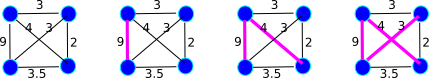
\includegraphics[width=5in]
{chow/spanning-tree.png}
\caption{
Example of finding MST (maximum spanning tree)} 
\label{fig-spanning-tree}
\end{figure}

\begin{figure}[h!]
\centering
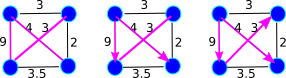
\includegraphics[width=3in]
{chow/tree-dir.png}
\caption{Example of giving directions
to edges of spanning tree.} 
\label{fig-tree-dir}
\end{figure}

Nodes in a Chow-Liu tree can
be rated in
terms
of their relative importance.
Here are 2 possible
metrics
for measuring 
the importance
of a node $\rva$:

\beq
N_{nb}(\rva)=
\text{ number of neighbors of $\rva$}
\eeq

\beq
{\rm traffic}(\rva)=
\sum_{\rvn\in nb(\rva)}
H(\rva:\rvn)
\eeq
For example,
to get a tree with low depth, 
one can choose
as the root node
the node which has 
largest $N_{nb}$, and
if there are several
with the same largest $N_{nb}$,
choose out of those the 
one with the largest traffic.


\section{Tree Augmented Naive Bayes (TAN)}

Recall from Chapter \ref{ch-naive}
that a Naive
Bayes bnet
consists
of  a class node $\rvc$
with
$n$ children nodes
$\rvx^n$, called the feature nodes. A
Tree Augmented Naive Bayes (TAN) bnet
is a Naive Bayes bnet with 
a 
tree grafted onto it like a chimera.
More precisely,
one starts
with a Naive Bayes bnet 
and adds arrows between
the feature nodes.
The arrows are added in such a way
that the TAN bnet sans node $\rvc$
constitutes a tree.
It's not the most well 
motivated bnet in human
history,
but at least
it adds a bit
of correlation between
the feature nodes
of the Naive Bayes bnet.
Those nodes are independent
at fixed $\rvc$
in the Naive Bayes
bnet, but are no longer so
in the TAN bnet.
See Figs.\ref{fig-naive-tree}
and \ref{fig-tan}
for an example of a TAN bnet.



\begin{figure}[h!]
\centering
$$\xymatrix{
\rvc\ar[d]\ar[dr]\ar[drr]\ar[drrr]\\
\rvx_0&\rvx_1&\rvx_2&\rvx_3
}
\;\;\;\;
\xymatrix{
\rvx_0&\rvx_1
&\rvx_2\ar[l]\ar@/^1pc/[ll]
&\rvx_3\ar[l]
}$$
\caption{bnet for Naive Bayes
with 4 feature nodes
and another bnet for a tree
made of the same feature nodes.}
\label{fig-naive-tree}
\end{figure}

\begin{figure}[h!]
\centering
$$\xymatrix{
\rvc\ar[d]\ar[dr]\ar[drr]\ar[drrr]\\
\rvx_0&\rvx_1
&\rvx_2\ar[l]\ar@/^1pc/[ll]
&\rvx_3\ar[l]
}$$
\caption{
TAN bnet constructed
by merging Naive
Bayes bnet
and tree
bnet
of Fig.\ref{fig-naive-tree}.}
\label{fig-tan}
\end{figure}


The total probability distribution
$P_{TAN}$ for a TAN bnet
can be parameterized as follows.

\beq
P_{TAN}(x^n, c)=P_{TAN}(c)\prod_{i=0}^{n-1}
P_{TAN}(x_i|x_{\mu(i)}, c)
\;.
\eeq

As with Chow Liu trees,
we can attempt
to find a TAN bnet
whose total 
probability $P_{TAN}=P_{\rvt^n, \rvc}$
best approximates
an a priori given probability 
distribution $P=P_{\rvx^n, \rvc}$.

Note that
\begin{claim}

\beq
\argmin_\mu H(\rvx^n, \rvc)
=
\argmax_\mu
\sum_i H(\rvx_i:\rvx_{\mu(i)}| \rvc)
\eeq
\end{claim}
\proof

\begin{align}
H(\rvx^n, \rvc)
&=
-\sum_{x^n,c}P(x^n,c)
\left[
\ln P(c)+
\sum_i
\ln P(x_i|x_{\mu(i)}, c)
\right]
\\
&=
-\sum_{x^n,c}P(x^n,c)
\left[
\ln P(c)+
\sum_i
\ln \left(\frac{P(x_i, x_{\mu(i)}|c)}
{P(x_i|c)P(x_{\mu(x_i)}|c)}
P(x_i| c)
\right)
\right]
\\
&=
\sum_i H(\rvx_i, \rvc)
-
\sum_i H(\rvx_i:\rvx_{\mu(i)}|\rvc)
\end{align} 
\qed


Following
the same line of
reasoning
that we followed
for Chow-Liu trees,
we conclude that:

If $D_{KL}(P\parallel P_{TAN})$
is minimized over all $P_{TAN}$, then
\begin{enumerate}
\item$P_{TAN}$
inherits
its TPM's 
from $P$, and
\item
$P_{TAN}$ gets
its structure,
which is being parameterized
by 
the function $\mu$,
by
maximizing 
the score defined by

\beq
\text{score}
=\sum_i H(\rvx_i:\rvx_{\mu(i)}|\rvc)
\label{eq-score-tan}
\eeq
\end{enumerate}

One can build a TAN bnet
from empirical data as follows:

Calculate a Chow-Liu Tree
for each $c\in S_\rvc$.
For each of those trees,
create a TAN bnet, and 
calculate its
score given by
  Eq.(\ref{eq-score-tan}).
Keep
the TAN bnet with
the largest score.

